\documentclass[12pt,a4paper,spanish]{article}

\usepackage[utf8]{inputenc}
\pagestyle{headings}
\usepackage{babel}
\usepackage{xcolor}
\usepackage{amsmath}
\usepackage{amsfonts}
\usepackage{amssymb}
\usepackage[pdftex]{graphicx}
\usepackage[unicode=true] {hyperref}
\usepackage[toc, page, header]{appendix}

\makeatletter

%%%%%%%%%%%%%%%%%%%%%%%%%%%%%% LyX specific LaTeX commands.
\pdfpageheight\paperheight
\pdfpagewidth\paperwidth

\title{\textbf{RNAemo}\\ \vspace{0.45cm} Especificación de Diseño de Software} 
\author{Franco Gaspar Riberi}

\begin{document}
\maketitle\pagebreak{}\tableofcontents{}\pagebreak{}

\newpage

\section{Introducción}
\subsection{Propósito}

El propósito de este documento es la especificación de
diseño de software correspondiente a la primera versión del producto 
\emph{\textbf{RNAemo}}.

La confección de este documento se contextualiza dentro del desarrollo de la tesis
de grado de la carrera Licenciatura en Ciencias de la Computación de la UNRC,
\emph{\textbf{RNAemo}}, a cargo de Franco Gaspar Riberi, con la dirección
de la Lic. Laura Tardivo (UNRC) y las colaboracines de Daniel
Gutson, el Lic. Guillermo Biset y el Dr. Roberto Daniel Rabinovich
(\textbf{FuDePAN}).

El documento esta dirigido a las personas involucradas en el desarrollo de la
tesis como así también a todos los colaboradores de \textbf{FuDePAN} que eventualmente
podrían participar en las etapas de desarrollo y mantenimiento del software.

\subsection{Descripci\'on general del documento}
En la sección~\ref{consideraciones} se mencionan los objetivos, la
metodología adoptada y las dependencias del diseño.

En la sección~\ref{arquitectura} se exhibe la arquitectura general del
sistema con sus principales componentes e interacciones.

En la sección~\ref{high_level_design} se presenta el diseño de alto nivel del sistema,
sus interfaces y paquetes principales.
				    
En la sección~\ref{low_level_design} se observa el diseño de bajo nivel del sistema,
esto involucra las clases concretas y sus relaciones para cada paquete.

\section{Consideraciones de diseño}
\label{consideraciones}

\subsection{Objetivos}
Se pretende lograr un diseño del sistema que cumpla con los principios
fundamentales del diseño orientado a objetos, comúnmente conocidos por el
acrónimo \textbf{``SOLID''} \cite{martin}.

En particular, se pretenden respetar los principios \textbf{SRP}
(\textit{Single Responsability Principle}), \textbf{OCP} (\textit{Open-Closed
Principle}) y \textbf{DIP} (\textit{Dependency Inversion Principle})
debido a su importancia para obtener un sistema f\'acilmente extensible
y configurable con el fin de satisfacer las necesidades de los usuarios.
  
\subsection{Metodología}
La metodología empleada para realizar el análisis y descripción del
diseño se denomina \emph{``Diseño dirigido por responsabilidades''}\cite{rebecca}. 

Esta técnica se enfoca en \textit{qué} acciones
(responsabilidades) deben ser cubiertas por el sistema 
y que objetos serán los responsables de llevarlas a cabo.
\textit{Cómo} se realizara cada acción, queda en un segunda plano.

\subsection{Herramientas y convenciones}
Se utiliza UML\cite{uml} como lenguaje de modelado, ArgoUML\cite{argoUML}
como herramienta para la confección de diagramas, y Dia\cite{dia} para la edición
de diagramas de propósito general. Además se adopta la convención de nombrar a
 las interfaces anteponiendo una letra \textit{``I''} al nombre de la clase concreta
que la implementa. \\
Por ejemplo, interface: \textit{``IPersona''} $\to$
clase concreta: \textit{``Persona''}.

\section{Arquitectura del sistema}
\label{arquitectura}
La arquitectura del sistema y la interacción entre los diversos módulos que la conforman se exhiben en la figura~\ref{arquitecture}.	A continuación se describe brevemente cada uno de ellos.

\begin{itemize}
  \item \textbf{MasterOfPuppets:} corresponde al módulo principal en términos de ejecución del sistema. Comprenderá
  la inicialización e invocación de los demás componentes. Representa el módulo encargado de contabilizar y generar 
  las tablas y gráficos que se esperan como salida de este software. Tomará como inputs secuencias de $_m$$_i$RNA y  
  RNA$_m$ desde archivos en formato FASTA.

  \item \textbf{Generador:} representa el módulo encargado de la generación de secuencias humanizadas. Dada una 		 
  secuencia original, genera la secuencia humanizada de la misma. Dicho módulo es externo a este desarrollo, y para ello  
  se empleará el software \emph{GeneDesign}\footnote{Descarga de: 
  \textcolor{blue}{http://www.xmarks.com/site/slam.bs.jhmi.edu/gd/}}. %ver este link

  \item \textbf{Matcher:} representa el módulo encargado de realizar el matching por complemento y el cálculo de score
  entre secuencias de RNA$_m$ y small-RNA$_s$. 

  \item \textbf{RNAmData:} representa el módulo que provee al sistema las cadenas de RNA$_m$ correspondientes para su 	
  uso. Corresponderá a una interfaz permitiendo hacer trasparente el uso de diversas fuentes de mensajeros.

  \item \textbf{RNAmSequence:} representa la base de datos de RNA$_m$ a través de un archivo en formato FASTA.

  \item \textbf{BlastProxy:} corresponde a un módulo externo el cual permite el alineamiento de secuencias mediante BLAST. 	 Básicamente, compara una secuencia con una gran cantidad de secuencias administradas en una base de datos.

  \item \textbf{$_m$$_i$RNASequence:} corresponde a la base de datos de secuencias de small-RNA$_s$ a través de un archivo 	  en formato FASTA. (particularmente $_m$$_i$RNA).

  \item \textbf{fideo:} corresponde a una librería parcialmente ya implementada. Provee al sistema la funcionalidad de 
  \emph{``folding''}. Se deberán agregar los backends \textsf{UNAFold} y \textsf{MFold}.

  \item \textbf{Validator:} representa el módulo encargado de realizar el control de calidad del sistema. Es el componente 	 encargado de decidir, si una secuencia se encuentra en el marco de lectura correcto o no.

  \item \textbf{StatisticalControl:} representa el módulo encargado de realizar controles estadísticos sobre las 	 
  secuencias entrantes.

  \item \textbf{Outputs:} refiere a los archivos con formato \textsf{CSV} que serán obtenidos como resultado del presente
  producto.
 
\end{itemize}

\begin{figure}[!hbtp]
	\begin{center}
		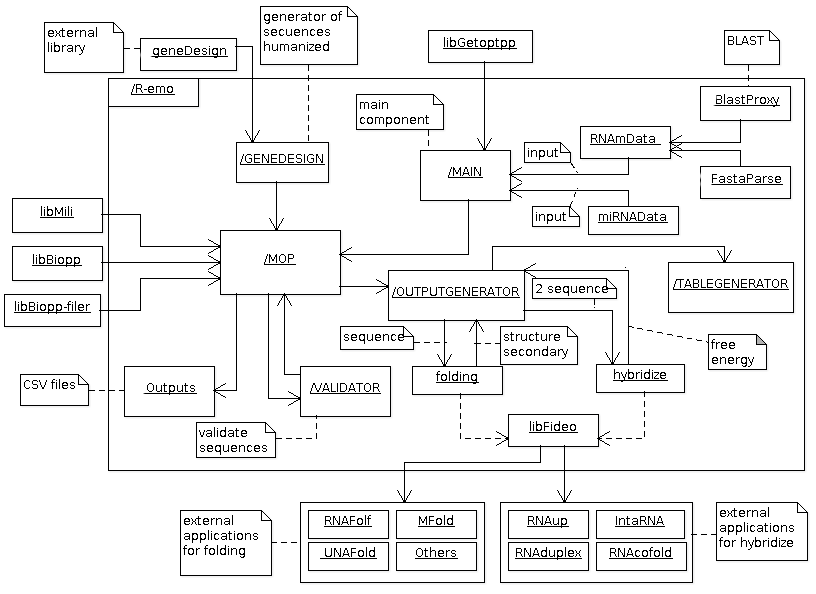
\includegraphics[width=20cm, height=12cm, angle=90]{arquitecture.png}
		\caption{UML - Arquitectura del Sistema}
		\label{arquitecture}
	\end{center}
\end{figure}

\section{Diseño de alto nivel}
\label{high_level_design}

\subsection{Interfaces - Responsabilidades - Colaboradores}
En esta sección se presentan las principales interfaces que intervienen en el sistema, sus respectivas responsabilidades y colaboradores. En la figura~\ref{interface} se exhibe el diagrama de interfaces correspondiente.

Finalmente, en la figura~\ref{mensajes} se presenta el diagrama de secuencia correspondiente a la comunicación entre las principales entidades del sistema.

\begin{figure}[!hbtp]
	\begin{center}
		\includegraphics[width=14cm,height=10.5cm]{interface.png}
		\caption{UML - Interfaces}
		\label{interface}
	\end{center}
\end{figure}

\subsubsection{IValidator}
\par \textbf{Responsabilidad:} Realizar el control de calidad para las secuencias. Determinar si una secuencia se encuentra en un marco de lectura válido o no. 

\par \textbf{Colaboradores:} biopp, bioedit
 
\subsubsection{IControlSeq}
\par \textbf{Responsabilidad:} Realizar el control estadístico sobre las secuencias.

\par \textbf{Colaboradores:}

\subsubsection{IFold}
\par \textbf{Responsabilidad:} Proveer al sistema el \emph{``folding''} de secuencias de RNA.

\par \textbf{Colaboradores:} \\
\hspace*{3.75cm} 1. Vienna Package (RNAFold). \\
\hspace*{3.75cm} 2. UNAFold. \\
\hspace*{3.75cm} 3. MFold. \\
\hspace*{3.75cm} 4. Otros.

\subsubsection{ISequence}
\par \textbf{Responsabilidad:} Provee al sistema el \emph{``matching''} de secuencias.
	
\par \textbf{Colaboradores:} fideo 

\subsubsection{IData}
\par \textbf{Responsabilidad:} Provee al sistema las secuencias de RNA$_m$.

\par \textbf{Colaboradores:} \\
\hspace*{3.75cm} 1. FastaParse \\
\hspace*{3.75cm} 2. ProxyBlast \\

\subsubsection{IHumanize}
\par \textbf{Responsabilidad:} Provee al sistema la \emph{``humanización''} de secuencias de RNA$_m$.
	
\par \textbf{Colaboradores:} geneDesign 

\begin{figure}
  \centering
  \includegraphics[scale=0.45, angle=90]{diagramaDeSecuencias.png}  
  \caption{UML - Pasaje de mensajes}
  \label{mensajes}
\end{figure}


\section{Diseño de bajo nivel}
\label{low_level_design}

\subsection{Paquetes y clases concretas}
En esta sección se presentan las clases concretas que implementan las interfaces presentadas en la 
sección~\ref{high_level_design}. Para mayor claridad, se dividieron los diagramas UML por paquetes.

\subsubsection{Validator}
\par En la figura ~\ref{validator} se exhibe el diagrama de clases correspondiente al componente \textsf{validator}. Este paquete representa el módulo ``Validator'' que se observa en la figura \ref{arquitecture} en la sección ~\ref{arquitectura}.

\par La responsabilidad de este componente es realizar un control de calidad sobre las secuencias de small-RNA$_s$ determinando si las mismas se encuentran en un marco de lectura válido. Para garantizar esta calidad, es necesario traducir la cadena de nucleótidos a una cadena de aminoácidos y verificar que no queden nucleótidos libres, conocidos como \emph{codones stops}. Para ello se utilizará la librería \emph{BioPP}.

\begin{figure}[!hbtp]
	\begin{center}
		\includegraphics[width=8cm,height=5.5cm]{validator.png}
		\caption{UML - Validator}
		\label{validator}
	\end{center}
\end{figure}

\subsubsection{StatisticalControl}
\par En la figura ~\ref{statisticalControl} se observa el diagrama de clases correspondiente al componente \textsf{statisticalControl}. El mismo representa el módulo ``StatisticalControl'' que se exhibe en la figura \ref{arquitecture} en la sección ~\ref{arquitectura}.

\par La responsabilidad de este componente radica en realizar controles estadísticos sobre las secuencias de RNA$_m$. Para estos controles, será necesario la generación de secuencias random.	

\begin{figure}[!hbtp]
	\begin{center}
		\includegraphics[width=7cm,height=5.5cm]{statisticalControl.png}
		\caption{UML - StatisticalControl}
		\label{statisticalControl}
	\end{center}
\end{figure}

\subsubsection{RNAmData}
\par En la figura ~\ref{RNAmData} se observa el diagrama de clases correspondiente al componente \textsf{RNAmData}. El mismo representa el módulo ``RNAmData'' que se exhibe en la figura \ref{arquitecture} de la sección ~\ref{arquitectura}.

\par Este componente corresponde a una interface que brinda al sistema las diversas secuencias de RNA mensajero. Permite utilizar diversas fuentes de datos, en primera instancia se abarcan dos fuentes; por un lado, \emph{fasta parser} que corresponde a un archivo en formato FASTA, y por el otro (a futuro), \emph{BlastProxy} que corresponde a la obtención de secuencias a través de BLAST.	

\begin{figure}[!hbtp]
	\begin{center}
		\includegraphics[width=6.5cm,height=5.5cm]{RNAmData.png}
		\caption{UML - RNAmData}
		\label{RNAmData}
	\end{center}
\end{figure}

\subsubsection{Matcher}
\par En la figura~\ref{matching} se observa el diagrama de clases para el paquete \textsf{Matcher}. Este paquete representa el componente \textsf{Matcher} correspondiente a la figura~\ref{arquitecture} de la sección~\ref{arquitectura}.
\par La responsabilidad de este componente es realizar el matching entre secuencias y calcular el score de matching. Para ello, se generarán diversas cadenas por cada posición del RNA$_m$ resultantes de matching diferentes. 

\begin{figure}[!hbtp]
	\begin{center}
		\includegraphics[width=7cm,height=5cm]{matching.png}
		\caption{UML - Matching}
		\label{matching}
	\end{center}
\end{figure}


\subsubsection{Generator}
	\textcolor{red}{\textbf{complete}}

\subsubsection{fideo}
\par En la figura~\ref{fideopackage} se observa el diagrama de clases para el paquete \textsf{fideo}. Este paquete representa el componente \textsf{fideo} correspondiente a la figura~\ref{arquitecture} de la sección~\ref{arquitectura}.
\par La responsabilidad de este componente es brindar al sistema el servicio de \emph{``folding''} sobre secuencias de RNA$_m$. Para cumplir con esta responsabilidad, se ofrece al sistema el acceso a librerías externas de manera transparente y
permitiendo utilizar diferentes librerías para acceder a diferentes servicios. 
\par Se contemplan los siguientes tipos de folding:
\begin{itemize}
	\item RNAFold.
	\item UNAFold.
	\item MFold.
\end{itemize}
\par La importancia de este paquete y las interfaces que contiene radica en que permite abstraerse del uso de una u otra librería.

\begin{figure}[!hbtp]
	\begin{center}
		
\includegraphics[width=8cm,height=6cm]{fideo.png}
		\caption{UML - fideo}
		\label{fideopackage}
	\end{center}
\end{figure}


\section{Fud-agnostic}
\label{fud}

\par El componente principal \textsf{MasterOfPuppets} será el encargado de la generación de las tablas. Para ello, se implementará un método \textsf{generateTable}, el cual tomará como parámetro el RNA mensajero, el RNA humanizado y un $_m$$_i$RNA. El componente principal realizará una doble iteración anidad entre RNA$_m$ y $_m$$_i$RNA. Es decir, por cada RNA$_m$ se recorrerá cada secuencia de $_m$$_i$RNA invocando al método ya mencionado.

\par Esto permitirá un paralelización trivial empleando \emph{FuD}.

\begin{center}
\textsf{generateTable (const Sequence\& rna\_original, const Sequence\& rna\_humanized, const Sequence\& mi\_rna)}
\end{center}



\begin{thebibliography}{99}
\small  \bibitem{martin} {\em{“Design Principles and Design Patterns.”}} 
		\textsc{Robert C. Martin}, 2000. \textcolor{blue}{http://www.objectmentor.com}
  
\small  \bibitem{rebecca} {\em{“Object Design: Roles, Responsibilities.”}} 
		\textsc{Rebecca Wirfs-Brock and Alan McKean and Collaborations}, Addison-Wesley, 2003.  

\small  \bibitem{uml} {\em{“Unified Modeling Language.”}} \textcolor{blue}{http://www.uml.org/}

\small  \bibitem{argoUML} {\em{“ArgoUML.”}} \textcolor{blue}{http://argouml.tigris.org/}

\small \bibitem{dia} {\em{“Dia.”}} \textcolor{blue}{http://live.gnome.org/Dia}
\end{thebibliography}

\end{document}
